\documentclass[landscape]{foils}
\usepackage[pdftex]{color}
\usepackage[pdftex]{graphicx}
\usepackage{eso-pic}
\usepackage[top=2cm, bottom=2cm, outer=0cm, inner=0cm]{geometry}
\usepackage{listings}
\usepackage{amsmath}
\usepackage{bold-extra}


\DeclareMathOperator{\sign}{sign}

% colors
\definecolor{DarkRed}{rgb}{0.5,0.0,0.0}
\definecolor{DarkBlue}{rgb}{0.0,0.0,0.35}
\definecolor{DarkGreen}{rgb}{0.0,0.6,0.00}
\definecolor{Orange}{rgb}{0.70,0.30,0.0}
\definecolor{Magenta}{rgb}{0.8,0.0,0.8}
\definecolor{DarkGray}{rgb}{0.3,0.3,0.3}
\definecolor{LightGray}{rgb}{0.9,0.9,0.9}
\definecolor{WhiteGray}{rgb}{0.99,0.99,0.99}
\definecolor{burgundy}{rgb}{0.667,0.110,0.094}
\def\burgundy{\color{burgundy}}
\def\red{\color{red}} 
\def\darkred{\color{DarkRed}} 
\def\blue{\color{DarkBlue}} 
\def\green{\color{DarkGreen}} 
\def\orange{\color{Orange}}
\def\magenta{\color{Magenta}}
\def\black{\color{black}}
\def\gray{\color{DarkGray}}
\def\shade{\color{LightGray}}
\def\hide{\color{WhiteGray}}

% sizes, footer and headers
\textwidth = 26truecm
\textheight = 18truecm
\topmargin =-2 cm
\oddsidemargin -1.5cm
\rightfooter{}
%
\def\indent{\hspace*{1cm}}
\def\prompt{\texttt{\$~}}
\def\prompt{{\footnotesize $\bullet$}~}
\def\exec#1{\indent\prompt\code{#1}}
\def\codeline#1{\indent\code{#1}}
\parindent 0pt

% alias for slides header
\def\Head#1{\foilhead{\burgundy #1 \vskip -1cm} \medskip\hrule\medskip}
\def\head#1{\foilhead{\burgundy #1 \vskip -1cm}}

% aliases for codes, files, namelists, etc.
\def\codecolor{\green}
\def\cardcolor{\orange}
\def\code#1{\texttt{\codecolor #1}}
\def\prog#1{\texttt{\burgundy #1}}
\def\var#1{\texttt{\burgundy #1}}
\def\file#1{\texttt{\green #1}}
\def\cmd#1{\texttt{\green #1}}
\def\nml#1{\texttt{\magenta #1}}
\def\card#1{\texttt{\cardcolor #1}}
\def\flag#1{\texttt{\green #1}}

% aliases for math
\def\vr{\ensuremath{\bm{r}}}
\def\vR{\ensuremath{\bm{R}}}
\def\vk{\ensuremath{\bm{k}}}
\def\vtau{\ensuremath{\bm{\tau}}}


\begin{document}

\blue
\vspace*{0.75cm}
\begin{center}

\includegraphics[width=0.45\textwidth]{../pictures/quantum_ogo_ok-1536x412.png}
\end{center}
~\\
%\vspace*{2cm}
%\MyLogo{~}
\vspace{0.80em}
\begin{center}
	\textbf{\burgundy \LARGE Advanced  {\scshape Quantum ESPRESSO} tutorial}\\[2em]
  {\burgundy\LARGE Day2: Basic PHONON  workflow}
  ~\\[1.3em]  
  \large Pietro Delugas
\end{center}

%%%%%%%%%%%%%%%%%%%%%%%%%%%%%%%%%%%%%%%%%%%%%%%%%%%%%%%%%%%%% 
\Head{Introduction to phonon workflows:}
\MyLogo{\burgundy {\bf Adv. QE 2023: Pavia Aug. 27 - Sept. 1}}
\rightheader{\hspace{-0.3cm}
\includegraphics[width=4.5cm]{../pictures/quantum_ogo_ok-1536x412.png}}

We will learn how to compute dynamical matrices, dielectric tensors, and vibrational modes and frequencies with \texttt{ph.x} 
Exercises: 
\begin{enumerate}
\item Computation of Zone Center phonons and dielectric tensors:
	\begin{itemize} 
		\item{Non polar case (fcc-Si) \file{Day2/PHONON/Exercise1.1/}}
		\item{Polar case (fcc AlAs) \file{Day2/PHONON/Exercise1.2/}}
	\end{itemize}
\item Calculation of phonons on $\mathbf{q}$-point meshes and Fourier Interpolation technique \file{Day-2/PHONON/Exercise2}:
	\begin{itemize}
	   \item{Calculation of phonon dispersion for fcc AlAs} 
           \item{Calculation of VDOS for fcc AlAs} 
	\end{itemize}
\end{enumerate}
    
%%%%%%%%%%%%%%%%%%%%%%%%%%%%%%%%%%%%%%%%%%%%%%%%%%%%%%%%%%%%% 
\head{About Quantum ESPRESSO}
More info about Quantum ESPRESSO can be found in:
\begin{itemize}
\item \file{https://www.quantum-espresso.org/}
\item Quantum ESPRESSO (QE) documentation:
  \begin{itemize}
  \item on-line manuals at
    \file{www.quantum-espresso.org/resources/users-manual}\\
    
  \item \file{Doc/} sub-directories in the {\sc Quantum ESPRESSO}
    distribution\\
    
  \item input data description: most programs contained in QE have
    their own input file description in the form of hyperlinked
    \file{\bf INPUT\_***.html} files (where \file{***} stands for the name
    of the program)
  \end{itemize}
\end{itemize}

%%%%%%%%%%%%%%%%%%%%%%%%%%%%%%%%%%%%%%%%%%%%%%%%%%%%%%%%%%%%%
\head{Hands-on material}

Hands-on material for these exercises is in \\ \file{/home/max/QuantumESPRESSO-school-2023/Day2/PHONON/}:
\vspace{-0.5em}
\begin{itemize}	
	\item \file{Exercise1.1} -- $\mathrm{\Gamma}$ modes for fcc-Si 
  \vspace{-0.5em}
\item \file{Exercise1.2/}   -- $\mathrm{Gamma}$ modes for fcc-AlAS 
  \vspace{-0.5em} 
\item \file{Exercise2}   -- Dispersion and VDOS for fcc-AlAs 
\end{itemize}


\begin{itemize}
\item All directories contain a \file{README.md} with instructions 
  how to run exercise(s)
\vspace{-0.5em}
\item To help recognizing for which program a given input file is
  intended, the filename starts with the name of the program, i.e.:
  \vspace{-0.5em}
\begin{itemize}
\item \file{<prefix>.scf*.in} -- input file for \prog{pw.x} program for the starting scf step 
\item \file{<prefix>.ph*.in} --  input file for \prog{ph.x} program for performing the DFPT calculations 
\item \file{<prefix>.<executable>.in} --input file for post-processing programs.  
\end{itemize}
\end{itemize}

{\burgundy {\bf Disclaimer:} {\em many examples use lousy convergence
    thresholds to speed-up calculations}}


%%%%%%%%%%%%%%%%%%%%%%%%%%%%%%%%%%%%%%%%%%%%%%%%%%%%%%%%%%%
\head{Reminder of conditions and definitions} 
\begin{itemize} 
\item Interatomic Force Constants: 
	\begin{itemize}
		\item Ground state is a structural local minimum: forces are vanishing; 
		\item We consider only small displacements around minimum:
			$$ \mathrm{\mathbf{R}_I} = \mathrm{\mathbf{R}^0_I} + \mathrm{\mathbf{u}_I} $$ 
	        \item  Forces have a linear dependence on small displacements: 
			$$ \mathrm{\mathbf{F}_I}(\{\mathrm{\mathbf{u}_I}\}) = -\sum_J{
				\frac{\partial^2{\mathrm{E}}}{\partial{\mathrm{\mathbf{u}_I}}\partial{\mathrm{\mathbf{u}_J}}}\cdot \mathrm{\mathbf{u}_J}
			} $$
		\item The set of force constants  $\mathrm{K}_{I,\alpha,J,\beta}$ thus  describes the dynamics of the harmonic system:  
			$$ \mathrm{K}_{I,\alpha,J,\beta}  = \frac{\partial^2{\mathrm{E}}}{\partial{\mathrm{u}_{I,\alpha}}\partial{\mathrm{u}_{J,\beta}}}$$
		\item Because of the periodicity we can rewrite $\mathrm{K}$ in a translationally invariant form:  
			$$ \mathrm{K}_{I_{\kappa},\alpha,J_{\sigma},\beta} = \mathrm{K}_{\kappa,\alpha,\sigma,\beta}(\mathrm{\mathbf{R}}_\kappa-\mathrm{\mathbf{R}}_\sigma)$$ 

	\end{itemize}
\end{itemize}
%%%%%%%%%%%%%%%%%%%%%%%%%%%%%%%%%%%%%%%%%%%%%%%%%%%%%%%%%%%%%%%%%
\head{Reminder of conditions and definitions}
\begin {itemize}
\item Monochromatic displaclemt patterns . 
	\begin{itemize}
		\item For infinite periodic systems it is necessary to decompose the dynamics into separate finite monochromatic modes: 
			$$ \tilde{\mathrm{\mathbf{u}}}(\mathbf{q}) i\cdot e^{i\mathbf{q}\cdot\mathbf{r}}$$ 	
		\item The generic monochromatic mode is described by the generalized amplitude:  
			$$\tilde{\mathrm{u}}_{\kappa,\alpha} = \sqrt{\mathrm{M}_{\kappa}}\mathrm{u}^0_{\kappa,\alpha} $$ 
			with $\kappa$ running on the atomic indexes of the lattice basis and $\alpha$ the cartesian indexes.
		\item  and a wavevector $\mathrm{\mathbf{q}}$ within the Brillouin zone  
        \end{itemize}
\end{itemize}
%%%%%%%%%%%%%%%%%%%%%%%%%%%%%%%%%%%%%%%%%%%%%%%%%%%%%%%%%%%%% 

\head{Reminder of conditions and definitions} 
\begin{itemize} 
		\item Dynamical matrices: 
\begin{itemize}
    \item At each $\mathbf{q}$  the equation of motion  are recast into a symmetric eigenvalue  problem for the generalized amplitude:   
	    $$ \sum_{\sigma,\beta}{D_{\kappa,\alpha;\sigma,\beta} \cdot \tilde{u}_{\sigma,\beta}} = \omega^2 \tilde{u}_{\kappa,\alpha} $$ 
    \item Where $\mathbf{D}$ is the mass symmetrized Fourier transform of the interatomic force constant matrix: 
	    $$ D_{\kappa,\alpha;\sigma,\beta}(\mathbf{q}) = \frac{1}{\sqrt{M_{\kappa}M_{\sigma}}} \sum_{\mathbf{R}}
		{K_{\kappa,\alpha,\sigma,\beta}(\mathbf{R}) e^{i \mathbf{q}\cdot{\mathbf{R}}}}$$ 
    \item Alternatively, more useful for plane-wave formalism,  the  dynamical matrices can be computed directly as mixed second derivatives of the energy with respect to 
	    the monochromatic displacements.   
\end{itemize}
\end{itemize}
%%%%%%%%%%%%%%%%%%%%%%%%%%%%%%%%%%%%%%%%%%%%%%%%%%%%%%%%%%%%%%%%%%%%%%%%%%%%%%%%%%%%%%%%%%%%%%%%%%%%
\head{Exercise 1: Calculation of Zone center phonons.}
We start computing the dynamical matrices and dielectric properties of fcc-Si
\begin{itemize} 
  \item Go to Exercise1.1 directory and start running the preliminary SCF calculation:\\[0.5em] 
	  \exec{cd Exercise1.1}\\
	  \exec{mpirun -np 2 pw.x < Si.scf.in > Si.scf.out }\\
  \item let's run our first phonon calculation:\\[0.5em]
	  \exec{mpirun -np 2 ph.x -i Si.phG.in > Si.phG.out} 
\end{itemize}
\vspace{1em}
\begin{center}
	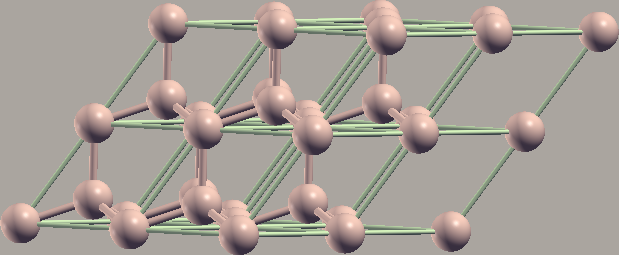
\includegraphics[width=14cm]{../pictures/fcc-Si.png}
\end{center}
%%%%%%%%%%%%%%%%%%%%%%%%%%%%%%%%%%%%%%%%%%%%%%%%%%%%%%%%%%%%%%%%%%%%%%%%%%%%%%%%%%%%%%%%%%%%%%%%%%%% 
\head{Exercise1.1 input}
\parbox{17cm}{
	\begin{itemize}
	\item \prog{ph.x} has only one namelist \var{\&inputph}
	\item \var{prefix} and \var{tmp} must match those used by \prog{pw.x} for the scf calculation. 
	\item \var{tr2\_ph} defines the convergence threshold for the self consistent solution of the Sternheimer equations. 
	\item \var{epsilon} asks the program to compute the Electric Field perturbation as well 
	\item \var{fildyn} defines the prefix for the files where the dynamical matrices are saved 
	\item After the namelist we indicate the coordinates of the wavevector for which we want compute the dynamical matrix. 
	\end{itemize}
}
\hskip 2cm
\parbox{8cm}{
\card{
    Phonons at Gamma \\
    \&inputph  \\
     prefix = 'Si'\, \\
     tr2\_ph = 1.0d-14, \\
     amass(1) = 28.0855, \\
     epsil = .true. \\
     outdir = './tmp' \\
     fildyn = 'Si.dyn', \\
    / \\
   0.0  0.0  0.0}
}
%%%%%%%%%%%%%%%%%%%%%%%%%%%%%%%%%%%%%%%%%%%%%%%%%%
\head{Exercise1.1 output} 
\prog{ph.x} writes types of output:
\begin{itemize}
	\item Standard output (\file{Si.phG.out}) with logging info and summary of the main results of the calculation. 
	\item Files with dynamical matrices (\file{Sy.dyn}) 
	\item Detailed data for recover and post-processing in \file{tmp/\_ph0/Si.phsave} directory. 
\end{itemize}
%%%%%%%%%%%%%%%%%%%%%%%%%%%%%%%%%%%%%%%%%%%%%%%%%%%%%%%%%%%%%%%%%%%%%%%%%%%%%%%%%%%%%%%%%%%%%%%%%%
\head{Exercise1.1 results}
Inspecting the content of \file{Si.phG.out} we find: \\
\parbox{12cm}{
\begin{itemize}
	\item {Symmetry analysys of the system, wavevector and summary of the perturnations that will be computed}
	\item {\shade log of the Self Consistent calculation of the density responses for each perturbation} 
	\item {\shade Summary of the general results}
\end{itemize}
}
\hskip 2cm  
\parbox{12cm}{
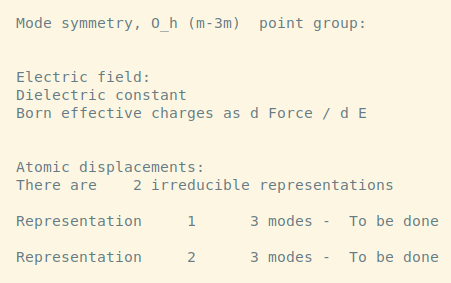
\includegraphics[width=11cm]{../pictures/Summary_simmetry_and_modes.png} 
}
%%%%%%%%%%%%%%%%%%%%%%%%%%%%%%%%%%%%%%%%%%%%%%%%%%%%%%%%%%%%%%%%%%%%%%%%%%%%%%%%%%%%%%%%%%%%%%%%%%
\head{Exercise1.1 results}
Inspecting the content of \file{Si.phG.out} we find: \\
\parbox{12cm}{
\begin{itemize}
	\item {\shade Symmetry analysys of the system, wavevector and summary of the perturnations that will be computed}
	\item {log of the Self Consistent calculation of the density responses for each perturbation} 
	\item {\shade Summary of the general results}
\end{itemize}
}
\hskip 2cm  
\parbox{12cm}{
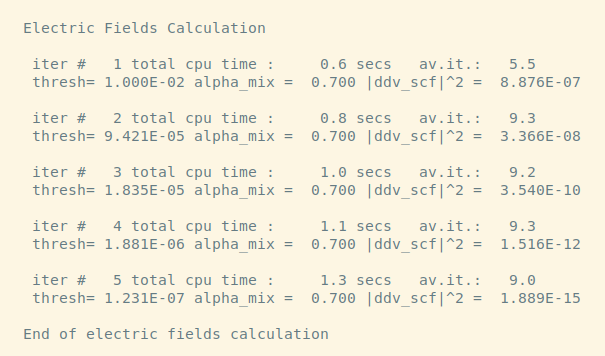
\includegraphics[width=11cm]{../pictures/SCF_log.png}  
}

%%%%%%%%%%%%%%%%%%%%%%%%%%%%%%%%%%%%%%%%%%%%%%%%%%%%%%%%%%%%%%%%%%%%%%%%%%%%%%%%%%%%%%%%%%%%%%%%%%
\head{Exercise1.1 results}
Inspecting the content of \file{Si.phG.out} we find: \\
\parbox{12cm}{
\begin{itemize}
	\item {\shade Symmetry analysys of the system, wavevector and summary of the perturnations that will be computed}
	\item {\shade log of the Self Consistent calculation of the density responses for each perturbation} 
	\item {Summary of the general results}
\end{itemize}
}
\hskip 2cm  
\parbox{12cm}{
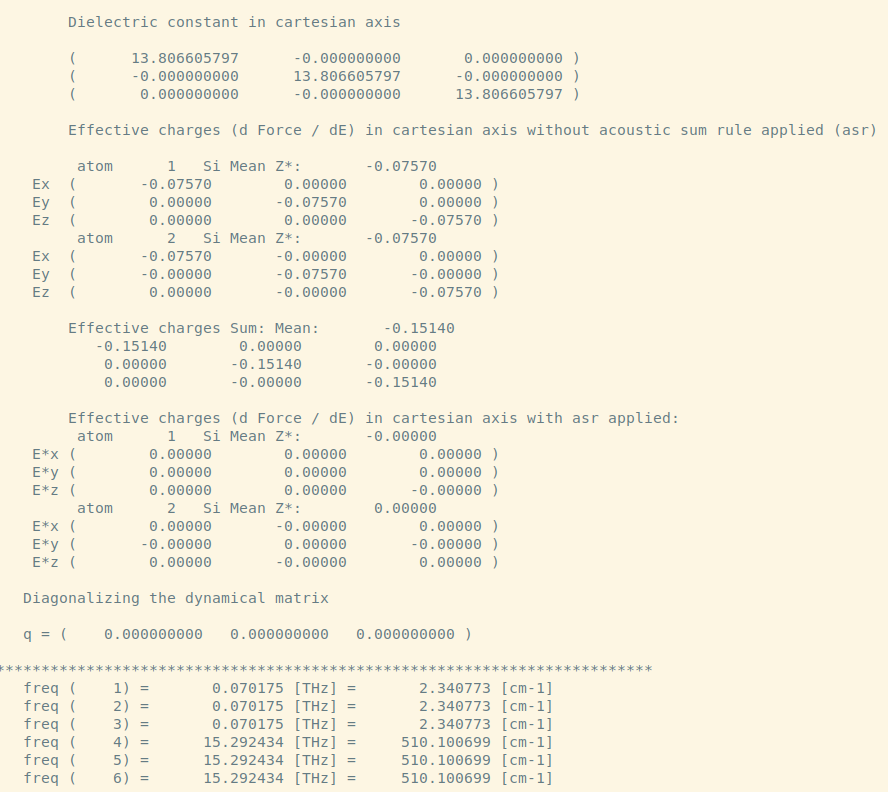
\includegraphics[width=12cm]{../pictures/summary_Si_phG.png} 
}
%%%%%%%%%%%%%%%%%%%%%%%%%%%%%%%%%%%%%%%%%%%%%%%%%%%%%%%%%%%%%%%%%%%%%%%%%%%%%%%%%%%%%%%%%%%%%%%%%%%%%%%%%%%%%%%
\head{Exercise1.1 results}
\begin{itemize}
\item The acustic sum rules for the rigid translations and for the Born Charges are not exaclty fullfilled. In the  next step we will see that 
	(if the deviation is small) we can correct them on the post-processing phase. It is also possible to obtain smaller deviation improving 
		the convergence of our ground state and perturbative calculations. 
	%\item {Rigid translation energies:
	%\begin{itemize}
	%	\item Use tighter thresholds for both \prog{pw.x} and \prog{ph.x} steps: set \var{conv\_thr} to 1.d-13 
	%		in \file{Si.scf.in} and \var{tr2\_ph} to 1.d-26 
	%		in \file{Si.phG.in} and repeat the calculation. 
	%	\item Use a finer FFT mesh increasing the cutoff: compare results with \var{ecutwfc} set to 30 40 and 50 Ry respectively.  
	%\end{itemize}
	%	}
	%\item {\hide Electric field perturbation is more sensitive to convergence w.r.t. the  k-point mesh used. In our case deviation from the
	%	ASR is significant, which usually means that also the dielectric tensor is inaccurate. Try to see what happens improving the k-point 
	%	sampling. 
	%	}
\end{itemize}
%%%%%%%%%%%%%%%%%%%%%%%%%%%%%%%%%%%%%%%%%%%%%%%%%%%%%%%%%%%%%%%%%%%%%%%%%%%%%%%%%%%%%%%%%%%%%%%%%%%%%%%%%%%%%%%%%%%%%%%%%%%%%%%%
\head{Exercise1.1 results}
\begin{itemize}
\item The acustic sum rules for the rigid translations and for the Born Charges are not exaclty fullfilled. In the  next step we will see that 
	(if the deviation is small) we can correct them on the post-processing phase. It is also possible to obtain smaller deviation improving 
		the convergence of our ground state and perturbative calculations. 
	\item {Rigid translation energies:
	\begin{itemize}
		\item Use tighter thresholds for both \prog{pw.x} and \prog{ph.x} steps: set \var{conv\_thr} to 1.d-13 
			in \file{Si.scf.in} and \var{tr2\_ph} to 1.d-26 
			in \file{Si.phG.in} and repeat the calculation. 
		\item Use a finer FFT mesh increasing the cutoff: compare results with \var{ecutwfc} set to 30 40 and 50 Ry respectively.  
	\end{itemize}
		}
	%\item {\hide Electric field perturbation is more sensitive to convergence w.r.t. the  k-point mesh used. In our case deviation from the
	%	ASR is significant, which usually means that also the dielectric tensor is inaccurate. Try to see what happens improving the k-point 
	%	sampling. 
	%	}
\end{itemize}
%%%%%%%%%%%%%%%%%%%%%%%%%%%%%%%%%%%%%%%%%%%%%%%%%%%%%%%%%%%%%%%%%%%%%%%%%%%%%%%%%%%%%%%%%%%%%%%%%%%%%%%%%%%%%%
\head{Exercise1.1 results}
\begin{itemize}

\item The acustic sum rules for the rigid translations and for the Born Charges are not exaclty fullfilled. In the  next step we will see that 
	(if the deviation is small) we can correct them on the post-processing phase. It is also possible to obtain smaller deviation improving 
		the convergence of our ground state and perturbative calculations. 
	\item {Rigid translation energies:
	\begin{itemize}
		\item Use tighter thresholds for both \prog{pw.x} and \prog{ph.x} steps: set \var{conv\_thr} to 1.d-13 
			in \file{Si.scf.in} and \var{tr2\_ph} to 1.d-26 
			in \file{Si.phG.in} and repeat the calculation. 
		\item Use a finer FFT mesh increasing the cutoff: compare results with \var{ecutwfc} set to 30 40 and 50 Ry respectively.  
	\end{itemize}
		}
	\item {Electric field perturbation is more sensitive to convergence w.r.t. the  k-point mesh used. In our case deviation from the
		ASR is significant, which usually means that also the dielectric tensor is inaccurate. Try to see what happens improving the k-point 
		sampling. 
		}
\end{itemize}

%%%%%%%%%%%%%%%%%%%%%%%%%%%%%%%%%%%%%%%%%%%%%%%%%%%%%%%%%%%%%%%%
\head{Exercise1.1: postprocessing with \prog{dynmat.x}} 
We now use \prog{dynmat.x} to refine our analysis. \\[0.05 em]
%\vskip 0.05 em
\exec{dynmat.x -i Si.dynmat.in > Si.dynmat.log} \\[0.05 em]
%\vskip 0.05 em
\parbox{16cm}{
\begin{itemize} 
	\item \var{fildyn} is used to indicate where the program finds the Dynamical matrix data, we put the name of the file just printed by \prog{ph.x}
	\item \var{asr} selects if enforcing  the ASR and how. 
	\item \var{lperm} is true if we want to printout the  dielectric tensor (electronic and ionic part) 
	\item \var{filout}, \var{filxsf}, etc. select the filename for saving displacements and frequencies in various formats. 
\end{itemize}
}
\hskip 2cm 
\parbox{8cm}{\small
	\card{
      \&input \\
      fildyn = 'Si.dyn',\\
      lperm = .true.\\
      asr = 'simple'\\
      filout = 'Si-dynmat.out'\\
      fileig = 'Si-dynmat.eig'\\
      filmol = 'Si-dynmat.mold'\\
      filxsf = 'Si-dynmat.xsf'\\
     /
	}\\
     \vskip 1.0em
     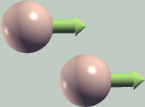
\includegraphics[width=3cm]{../pictures/Si-acustic.png} 
     \hskip 2em
     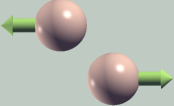
\includegraphics[width=3cm]{../pictures/Si-irrep2.png}
     }


%%%%%%%%%%%%%%%%%%%%%%%%%%%%%%%%%%%%%%%%%%%%%%%%%%%%%%%%%%%%%%%%%%%%%%%%%%%%%%%%%%
\head{Exercise1.2: AlAs Zone Center modes}
We now do the same exercise for fcc-AlAs: 
\begin{itemize}
	\item go to the working directory \\[0.5 em]
	 \exec{cd Day2/PHONON/Exercise1.2}
 \item run in sequence \prog{pw.x}, \prog{ph.x}, and \prog{dynmat.x} as in the previous exercise:\\[0.5 em] 
	\exec{mpirun -np 2 pw.x -i AlAs.scf.in > AlAs.scf.out}\\
	\exec{mpirun -np 2 ph.x -i AlAs.phG.in > AlAs.phG.out}\\
	\exec{dynmat.x -i AlAs.dynmat.in > AlAs.dynmat.log} \\
\item Now let us inspect files \file{AlAs.dyn} and \file{AlAs.dynmat.log} 
\end{itemize}
%%%%%%%%%%%%%%%%%%%%%%%%%%%%%%%%%%%%%%%%%%%%%%%%%%%%%%%%%%%%%%%%%%%%%%%%%%%%%%%%%%%% 
\head{Exercise1.2: Results} 
\parbox{16cm}{
	\begin{itemize}
	  \item Inspecting the dielectric tensors in \file{AlAs.dyn} we find that Born charges are now finite with 
		  a value of $\sim$ 2.15 for Al and -2.15 for As 
	  \item {\shade From \prog{\shade dynmat.x} output (\file{\shade AlAs.dynmat.log}) we find the 3 optical modes are Infrared active and they give a sizeable 
		  contribution to the static dielectric constant tensor.} 
	  \item {\shade The dielectric tensor mantains the cubic symmetry because the 3 optical modes for a degenerate triplet with mutually orthogonal
		  dipole directions.} 
	\end{itemize}
}
\hskip 2cm
\parbox{8cm}{
	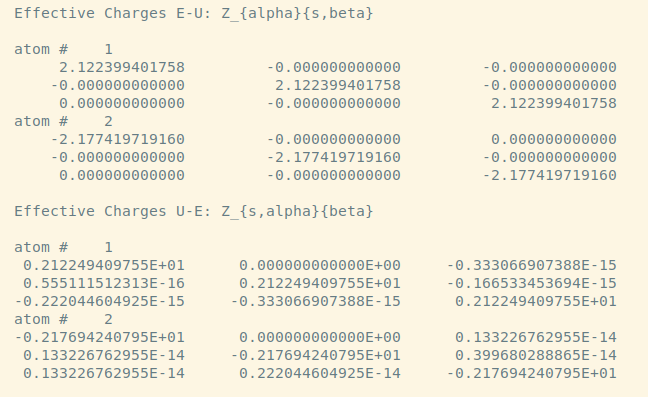
\includegraphics[width=8cm]{../pictures/AsAl_Born_charges.png}
}
%%%%%%%%%%%%%%%%%%%%%%%%%%%%%%%%%%%%%%%%%%%%%%%%%%%%%%%%%%%%%%%%%%%%%%%%%%%%%%%%%%%%
\head{Exercise1.2: Results} 
\parbox{16cm}{
	\begin{itemize}
		\item {\shade Inspecting the dielectric tensors in \file{\shade AlAs.dyn} we find that Born charges are now finite with 
			a value of $\sim$ 2.15 for Al and -2.15 for As} 
	  \item {From \prog{dynmat.x} output (\file{AlAs.dynmat.log}) we find the 3 optical modes are Infrared active and they give a sizeable 
		  contribution to the static dielectric constant tensor.} 
	  \item {\shade The dielectric tensor mantains the cubic symmetry because the 3 optical modes for a degenerate triplet with mutually orthogonal
		  dipole directions.} 
	\end{itemize}
}
\hskip 2cm
\parbox{8cm}{
	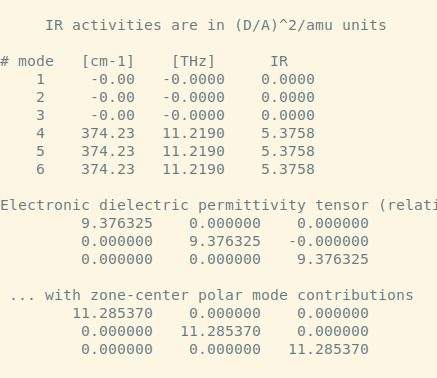
\includegraphics[width=8cm]{../pictures/polar_modes_AlAs.png}
}
%%%%%%%%%%%%%%%%%%%%%%%%%%%%%%%%%%%%%%%%%%%%%%%%%%%%%%%%%%%%%%%%%%%%%%%%%%%%%%%%%%%%
\head{Exercise1.2: Results} 
\parbox{16cm}{
	\begin{itemize}
		\item {\shade Inspecting the dielectric tensors in \file{\shade AlAs.dyn} we find that Born charges are now finite with 
			a value of $\sim$ 2.15 for Al and -2.15 for As} 
	  \item {From \prog{dynmat.x} output (\file{AlAs.dynmat.log}) we find the 3 optical modes are Infrared active and they give a sizeable 
		  contribution to the static dielectric constant tensor.} 
	  \item {The dielectric tensor mantains the cubic symmetry because the 3 optical modes for a degenerate triplet with mutually orthogonal
		  dipole directions.} 
	\end{itemize}
}
\hskip 2cm
\parbox{8cm}{
	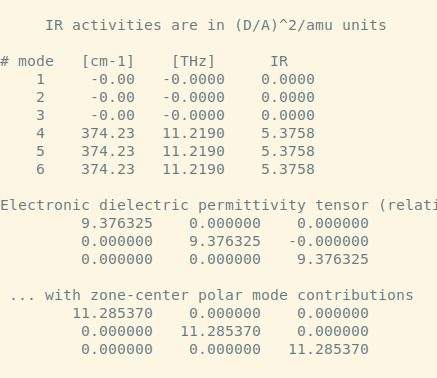
\includegraphics[width=8cm]{../pictures/polar_modes_AlAs.png}
}
%%%%%%%%%%%%%%%%%%%%%%%%%%%%%%%%%%%%%%%%%%%%%%%%%%%%%%%%%%%%%%%%%%%%%%%%%%%%%%%%%%%%
\head{Exercise1.2: evaluate the LO-TO splitting} 
(\small We now use \prog{dynmat.x} and the data in $\Gamma$ dynamical matrix to  estimate
the long wave limit of the the IR active phonons. We use the modified input \file{AlAs.dynmat-LO-TO.in}:\\[0.5em]
\exec{dynmat.x -i AlAs.dynmat-LO-TO.in > AlAs-dynmat-LO-TO.log}\\[3.5em]
\parbox{13cm}{\small
	\begin{itemize}
		\item To evaluate the splitting we need to specify a direction with 
			\var{q(1}, \var{q(2)}, and \var{q(3)}. 
		\item  In this case any direction is equivalent, the LO mode has a dipole oriented in the 
			selected direction. 
		\item  The LO~-~TO splitting is the one expected by the \\ Lyddane-Sachs-Teller relation: 
			$$ \omega_{LO} = \sqrt{\frac{\epsilon_0}{\epsilon_{\infty}}} \cdot \omega_{TO} = \sqrt{\frac{11.3}{9.4}}\cdot 374 = 410 $$ 
	\end{itemize}
	}
\hskip 2cm 
\parbox{10cm}{
	\card{\small
		\&input \\
    		fildyn = 'AlAs.dyn',\\
    		asr='simple',  \\	
    		amass(1)=26.98, \\
    		amass(2)=74.92\\
    		filout='AlAs-dynmatLOTO.out'\\
    		fileig='AlAs-dynmatLOTO.modes'\\
    		filmol='AlAs-dynmatLOTO.mold'\\
    		filxsf='AlAs-dynmatLOTO.xsf'\\ 
    		q(1) = 1.0, \\
    		q(2) = 1.0, \\
    		q(3) = 0.0  \\
 	/
	}
}
%%%%%%%%%%%%%%%%%%%%%%%%%%%%%%%%%%%%%%%%%%%%%%%%%%%%%%%%%%%%%%%%%%%%%%%%%%%%
\head{Exercise2: phonon dispersion in fcc-AlAs} 
In this exercise we will compute the phonon dispersion and the VDOS of AlAs. 
The material for this exercise is in \file{../../Day2/PHONON/Exercise2} directory. 
First step will be computing the dynamical matrices for a uniform mesh of wavevectors with \prog{ph.x}

\begin{itemize} 
	
	\item We first execute the scf calculations:\\
		\exec{mpirun -np 2 pw.x -i AlAs.scf.in > AlAs.scf.out}\\ 
	\item We now execute the phonon calculation, as we are running the calculation for many  $\mathbf{q}$s it is usually more efficient 
		to use the image parallelism as much as possible: \\
	        \exec{mpirun -np 2 ph.x -ni 2 -i AlAs.ph.in > AlAs.ph\_images.out} \\ 
	\item After using the image parallelism one has to execut a further single image \prog{ph.x} run to collect data and print the dynamical matrices. 
		\begin{itemize}
		 	\item Check that \var{recover} is set to \value{.true.} in \file{AlAs.ph.in}
			\item Execute with a  single image the recover run:\\
				\exec{mpirun -np 2 ph.x -i AlAs.ph.in > AlAs.ph\_recover.out}  
		\end{itemize}
	\end{itemize}

%%%%%%%%%%%%%%%%%%%%%%%%%%%%%%%%%%%%%%%%%%%%%%%%%%%%%%%%%%%%%%%%%%%%%%%%%%%%%%%%%%%%%%%%%%%%%%%%%%%%%%%%%%%%%%%%%%%
\head{Exercize2: Phonon input}
\vskip 4em
\parbox{16cm}{
	\begin{itemize}
		\item We \var{ldisp}  to  \value{.true.} to activate the calculation on a uniform mesh
		\item \var{nq1}, \var{nq2}, and \var{nq3} are used to set the uniform mesh used.
		\item Symmetries will be used to reduce the number of $\mathbf{q}$ computed. 
		\item \var{recover} must be set to \value{.true.} whenever  restarting the calculation.
		\item \var{fildyn} in this case indicates the suffix for the dynamical matrix files, a separate
			file will be produced for each q-point computed. 
	\end{itemize}
	}
\hskip 2cm
\parbox{8cm}{
	\card{
	Phonons on uniform q-grid\\
 	\&inputph\\
  	prefix='AlAs',\\  
  	tr2\_ph = 1.0d-14,\\
  	recover = .false.\\
  	ldisp = .true.,\\
  	nq1 = 4\\
  	nq2 = 4\\
  	nq3 = 4\\
   	outdir='./tmp'\\
  	fildyn='AlAs.dyn',\\
 	/}
}
%%%%%%%%%%%%%%%%%%%%%%%%%%%%%%%%%%%%%%%%%%%%%%%%%%%%%%%%%%%%%%%%%%%%%%%%%%%%%%%%%%%%%%%%%%%%%%%%%%%%%%%%%%%%%%%%%%%
\head{~\\[-0.4em] Exercise 2: Fourier interpolation of dynamical matrices }
\vskip 2 cm
\parbox{14cm}{
	\begin{itemize}
		\item We use the dynamical matrices on the $\mathrm{nq}_1 \times \mathrm{nq}_2 \times \mathrm{nq}_3$ 
			mesh to generate the force constants for a 
			$\mathrm{nq}_1 \times \mathrm{nq}_2 \times \mathrm{nq}_3$ supercell. \\[1em]
			\exec{q2r.x -i AlAs.q2r.in > AlAs.q2r.log} \\ 
		\item  We need to specify the suffix of the dynamical matrix files in \var{fildyn}
		\item  The force constants are saved in the file specified by \var{flfrc}.  
	\end{itemize}
}
\hskip 2cm
\parbox{8cm}{
	\card{\\
       \&input
	fildyn='AlAs.dyn',\\
        zasr='simple',\\ 
        flfrc='AlAs444.fc'\\
 /
	}
}
%	\item With the dynamical matrices and dielectric tensors  computed above we compute the interatomic force constants using \prog{q2r.x}:\\
%		\exec {q2r.x -i AlAs.q2r.in > AlAs-q2r.log} 
%	\item With the interatomic force constants we now compute the phonon dispersion and the VDOS using \prog{matdyn.x}:\\
%		\exec{matdyn.x -i AlAs.matdyn\_with\_labels.in > AlAs.matdyn\_dispersion.log} \\
%		\exec{matdyn.x -i AlAs\_dos.in > AlAs\_matdyn\_dos.log} \\ 
%	
%\end{itemize}
%%%%%%%%%%%%%%%%%%%%%%%%%%%%%%%%%%%%%%%%%%%%%%%%%%%%%%%%%%%%%%%%%%%%%%%%%%%%%%%%%%%%%%%%% 
\head{Exercise 2: Fourier interpolation}

\begin{itemize}
	\item Fourier transforming back  the force constants we estimate the dynamical matrices at any $\mathbf{q}$  
force constants.
  \item The long-range dipole-dipole interaction has been removed by \prog{q2r.x} 
	  and will be readded by \prog{matdyn.x}. 
  \item  The range of the remaing ion-ion interaction is assumed to be shorter than the chosen supercell. 
\end{itemize}
\vskip 1em
\parbox{12cm}{\small
  \begin{itemize}
	  \item We first compute the  phonon dispersion\\[0.5em]
	    \exec{matdyn.x -i AlAs.matdyn.in} \\[-1.0em] 
    \item For the dispersion we set \var{q\_in\_band\_form} to 
	    \value{.true.} and use band form for indicating the BZ path. 
    \item {coordinates can be indicated in $2\pi/a$ units, or setting \var{q\_in\_cryst\_coord} to \value{.true.} 
	   in fractional coordinated of the reciprocal lattice.}
    %\item {\hide or directly using special labels; using \var{\hide point\_label\_type} flag one can chose between the  
    %		   notation of Setyawan-Curtarolo   paper  (\value{\hide 'SC'}) or the Bilbao Crystallographic one (\value{\hide 'BI'})}
    
  \end{itemize}
	}
\hskip 4cm 
\parbox{9cm}{\small
	\card{
	\&input\\
    	asr = 'simple'\\            
    	q\_in\_band\_form = .true.\\ 
    	flfrc='AlAs444.fc',\\           
    	flfrq='AlAs\_dispersion.freq'\\
 /\\
 6\\
   0.00 0.00  0.00 18\\
   0.75 0.75  0.00 22\\
   0.50 1.00  0.00 17\\
   0.00 1.00  0.00 34\\
   0.00 0.00  0.00 29\\
   0.50 0.50  0.50  1
	}
	}
%%%%%%%%%%%%%%%%%%%%%%%%%%%%%%%%%%%%%%%%%%%%%%%%%%%%%%%%%%%%%%%%%%%%%%%%%%%%%%%%%%%%%%%%%%%%%%%5
\head{Exercise 2: Fourier interpolation}

\begin{itemize}
	\item Fourier transforming back  the force constants we estimate the dynamical matrices at any $\mathbf{q}$  
force constants.
  \item The long-range dipole-dipole interaction has been removed by \prog{q2r.x} 
	  and will be readded by \prog{matdyn.x}. 
  \item  The range of the remaing ion-ion interaction is assumed to be shorter than the chosen supercell. 
\end{itemize}
\vskip 1em
\parbox{12cm}{\small
  \begin{itemize}
	  \item We first compute the  phonon dispersion\\[0.5em]
	    \exec{matdyn.x -i AlAs.matdyn.in} \\[-1.0em] 
    \item For the dispersion we set \var{q\_in\_band\_form} to 
	    \value{.true.} and use band form for indicating the BZ path. 
    %\item {coordinates can be indicated in $2\pi/a$ units, or setting \var{q\_in\_cryst\_coord} to \value{.true.} 
    %	   in fractional coordinated of the reciprocal lattice.}
    \item {or directly using special labels; using \var{point\_label\_type} flag one can chose between the  
     notation of Setyawan-Curtarolo   paper  (\value{'SC'}) or the one of Bilbao Crystallographic Server (\value{'BI'})}
    
  \end{itemize}
	}
\hskip 4cm 
\parbox{9cm}{\small
	\card{
    \&input\\
    asr = 'simple'\\            
    q\_in\_band\_form = .true.\\ 
    flfrc='AlAs444.fc',\\           
    flfrq='AlAs\_dispersion.freq'\\
    point\_label\_type = 'SC'\\
 /\\
 6\\
   gG 18\\
   K  22\\
   W  17\\
   X  34\\
   gG 29\\
   L  1
		}
	}
%%%%%%%%%%%%%%%%%%%%%%%%%%%%%%%%%%%%%%%%%%%%%%%%%%%%%%%%%%%%%%%%%%%%%%%%%%%%%%%%%%%%%%%%%%%%%%%%%%%%%%%%%%%%%%
\head{Exercise 2: Fourier interpolation}

\begin{itemize}
	\item Fourier transforming back  the force constants we estimate the dynamical matrices at any $\mathbf{q}$  
force constants.
  \item The long-range dipole-dipole interaction has been removed by \prog{q2r.x} 
	  and will be readded by \prog{matdyn.x}. 
  \item  The range of the remaing ion-ion interaction is assumed to be shorter than the chosen supercell. 
\end{itemize}
\vskip 1em
\parbox{13cm}{\small
  \begin{itemize}
	  \item We then compute the  VDOS\\[0.5em]
	    \exec{matdyn.x -i AlAs\_dos.matdyn.in} \\[-1.0em] 
    \item For the VDOS  we set \var{dos} to  \value{.true.} and indicate 
	    values for k-mesh with \var{nk1}, \var{nk2}, \var{nk3}, and \var{deltaE} for 
		  the VDOS step 
    \item {remember to rename all printout files and indicate with \var{fldos} a filename for the VDOS printout}
    
  \end{itemize}
	}
\hskip 4cm 
\parbox{9cm}{\small
	\card{
    \&input\\
    asr = 'simple'\\            
    dos = .true. \\
    deltaE = 1.0 \\
    flfrc='AlAs444.fc',\\           
    nk1 = 8 \\
    nk2 = 8 \\
    nk3 = 8\\ 
    flfrq = 'AlAs\_dos.freq'\\
    flvec = 'AlAS\_dos.modes'\\
    fleig = 'AlAS\_dos.eig'\\
    fldos = 'AlAs\_vdos'\\
 / 
		}
	}



\end{document}

%%% Local Variables:
%%% mode: latex
%%% TeX-master: t
%%% End:
